\section{Ergebnisse}
In diesem Kapitel sind Versuchsergebnisse dargestellt, die an dem geregelten Pendel gewonnen wurden. Dafür wurde, das stabilisierte Pendel mit einem kurzen Störimpuls beaufschlagt und die Reaktion aufgezeichnet. Dieser Störimpuls erfolgte per Hand und wurde in unterschiedlichen Stärken durchgeführt, um so die einzelnen Controller testen zu können. 
\subsection{Swing-Up}
\begin{figure}[htbp]
	\label{fig.Swing-Up-Plot}
	\centering
	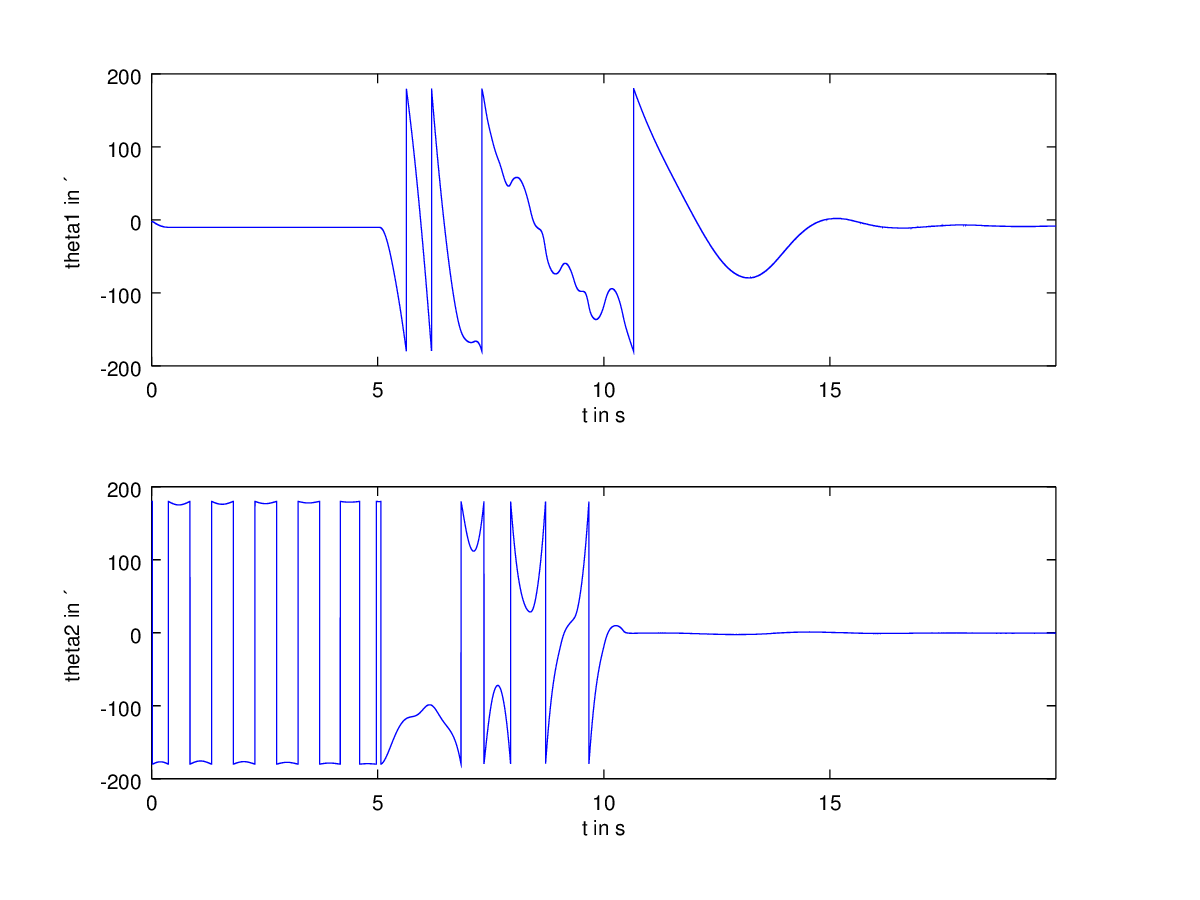
\includegraphics[width=1.\textwidth]{Grafiken/Swing-Up_kurz.png}
	\caption{Der Swing-Up-Vorgang}
\end{figure}

\subsection{Stabilisierer}
\begin{figure}[htbp]
	\label{fig.Stabilisierer-Plot}
	\centering
	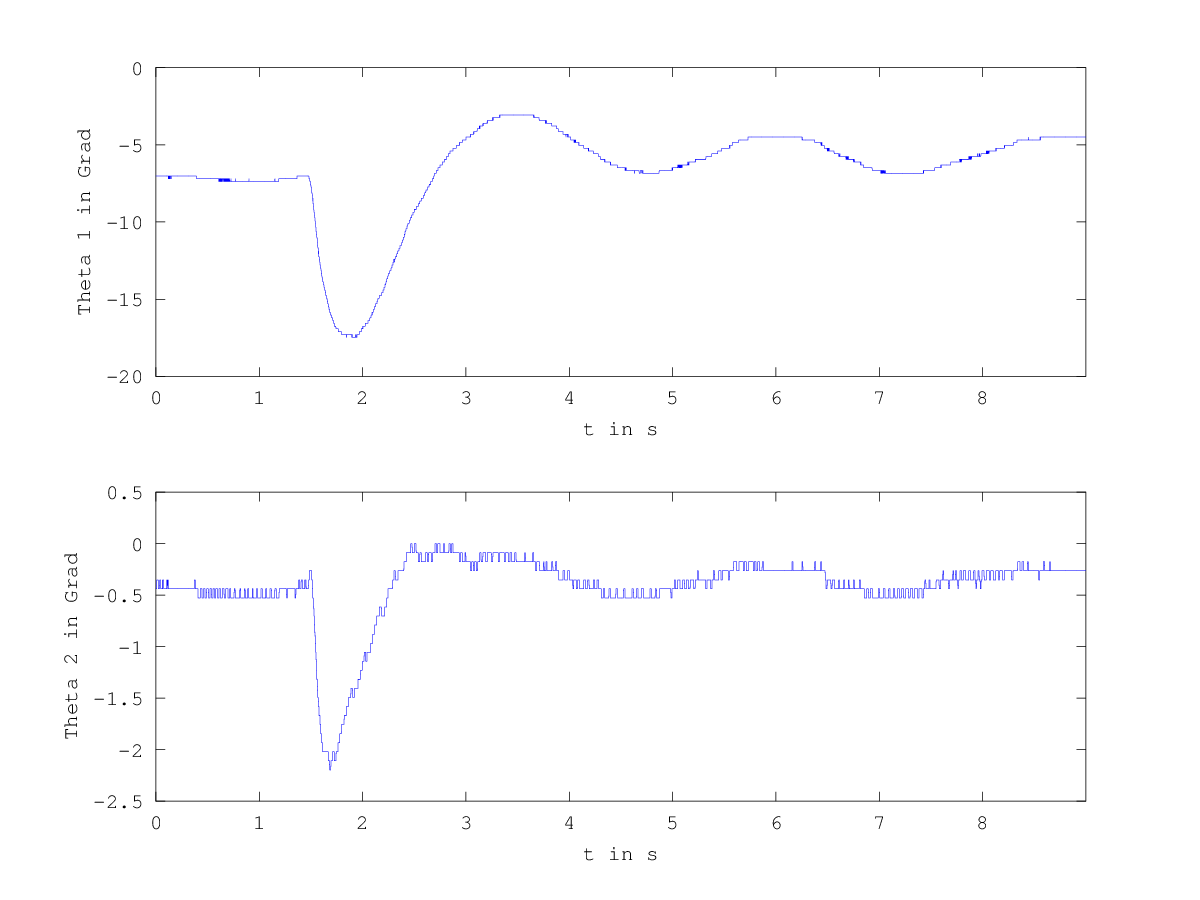
\includegraphics[width=1.\textwidth]{Grafiken/Stab_lang.png}
	\caption{Störung \textless $5^{\circ}$}
\end{figure}

\subsection{Catcher}
\begin{figure}[htbp]
	\label{fig.Catcher-Plot}
	\centering
	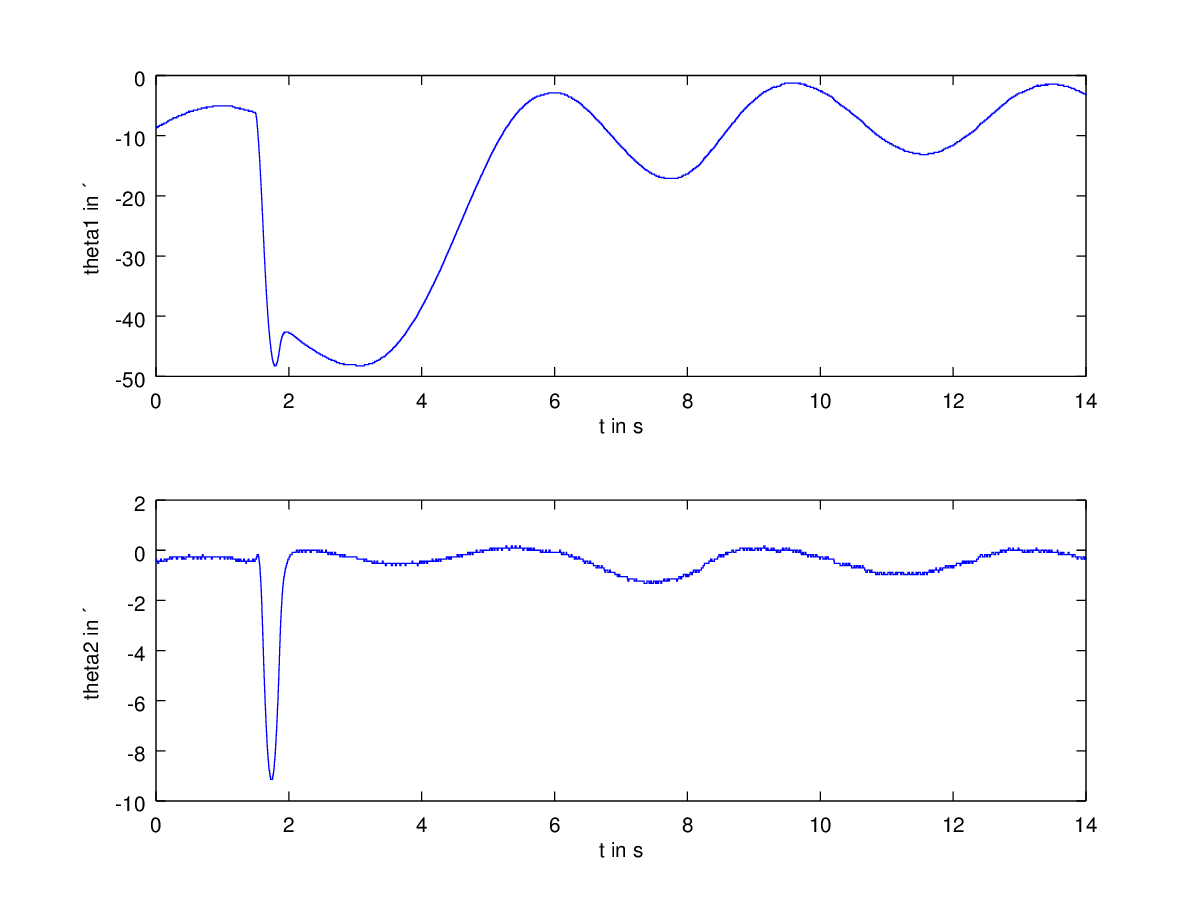
\includegraphics[width=1.\textwidth]{Grafiken/Catch_kurz.png}
	\caption{Störung \textgreater $5^{\circ}$}
\end{figure}

\subsection{Watchdog}
\colorbox{yellow}{Hier habe ich echt wenig Ahnung von!}
\begin{figure}[htbp]
	\label{fig.Watchdog-Plot}
	\centering
	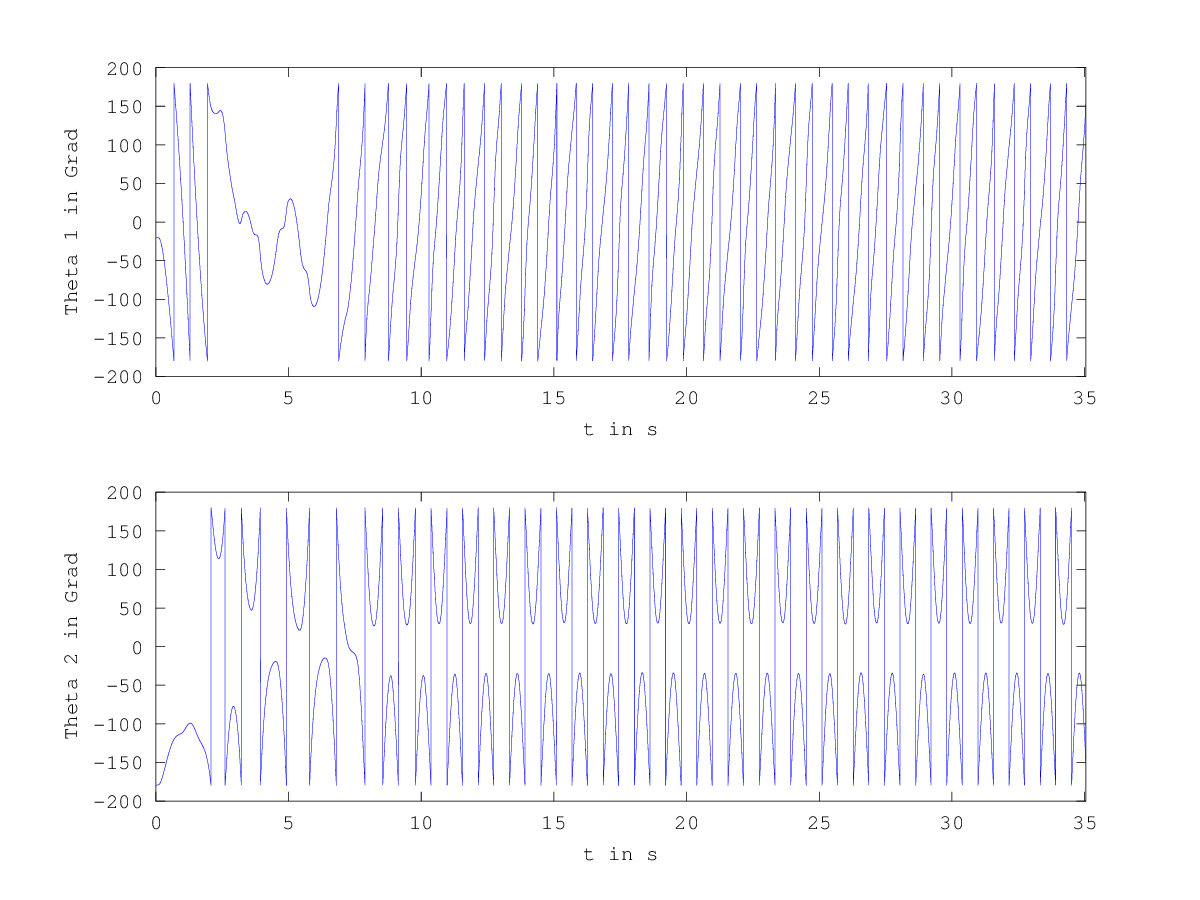
\includegraphics[width=1.\textwidth]{Grafiken/Watchdog_lang.png}
	\caption{Watchdog}
\end{figure}